% A two-column news report. Heading spanning two columns. Page size roughly A3. A figure and Subheading at neck.
% This code was written during 2008-2015 for Kolkata based Bengali fortnightly Khoborer Kagoj Songbadmanthan.
%============================================
\documentclass{article} 
\usepackage{fontspec} 
\usepackage{xunicode} 
\usepackage{xltxtra} 
\usepackage{multicol} 
\usepackage{ragged2e} 
\usepackage{wrapfig} 
\usepackage{graphicx} 
\usepackage{tikz}
\usetikzlibrary{shadows}
\usetikzlibrary{shapes,snakes}
\usepackage[papersize={11in,18in},top=1in,bottom=1.5in,left=0.5in,right=0.5in]{geometry} 
\usepackage{caption}
\captionsetup{singlelinecheck=false, format=plain, aboveskip=2pt, belowskip=1pt, margin=0pt, labelformat=empty, labelsep=none, justification=justified}
\definecolor{Light}{gray}{0.8}
\definecolor{Dark}{gray}{0.2}
\definecolor{Grey}{gray}{0.65}
%
% These are the fonts and their variations. Baban12 and BabanBold12 fonts are custom made. Font files are provided in the directory. Ubuntu font is available in internet freely. NOTE : Left quote is broken in the fonts, replaced by custom made left quote at চ্ছ্র 
\newcommand\EN[1]{	 
\fontsize{#1}{#1}\fontspec{Ubuntu}} 
\newcommand\BN[1]{ % Normal face of the Bengali font
\fontsize{#1}{#1}\fontspec[Script=Bengali]{Baban12}} 
\newcommand\BB[1]{ % Bold face of the Bengali font
\fontsize{#1}{#1}\fontspec[Script=Bengali]{BabanBold12}} 
\newcommand\BI[1]{ % Italic face of the Bengali font
\fontsize{#1}{#1}\fontspec[Script=Bengali, FakeSlant=0.2]{Baban12}} 
\newcommand\BBI[1]{ % Bold italic face of the Bengali font
\fontsize{#1}{#1}\fontspec[Script=Bengali, FakeSlant=0.2]{BabanBold12}} 
%
%
\begin{document}
% 
\begin{minipage}[t]{124mm} % A single news item should be within a minipage environment
\vspace{2mm}
\setlength{\baselineskip}{2pt}
\setlength{\parskip}{0.15ex} 
\setlength{\parindent}{10pt}
\begin{multicols}{2} % Two Column environment starts
[\section*{\Centering 
\BB{29.22}মেয়েটাকে পালিয়ে যেতে বলেছিল আটক চারজন, চ্ছ্রআসল দোষী' পলাতক\\[1.5mm]
}]
% following three lines for adjusting multiple columns. 
\setcounter{columnbadness}{7000}
\setcounter{finalcolumnbadness}{7000}
\tolerance=2000 
%
%
\begin{wraptable}[21]{r}[25mm]{50mm} % Neck subheading and figure environment starts here
\vspace{-6mm}
\rule{52mm}{1pt}\\[-1.5mm]
\BN{23.212}আকড়ার তরুণী নিগ্রহ\\[-5.5mm] % Neck subheading
\rule{52mm}{1pt}\\
\Centering
\setlength{\fboxsep}{0pt}
\setlength{\fboxrule}{0.05pt} \fbox{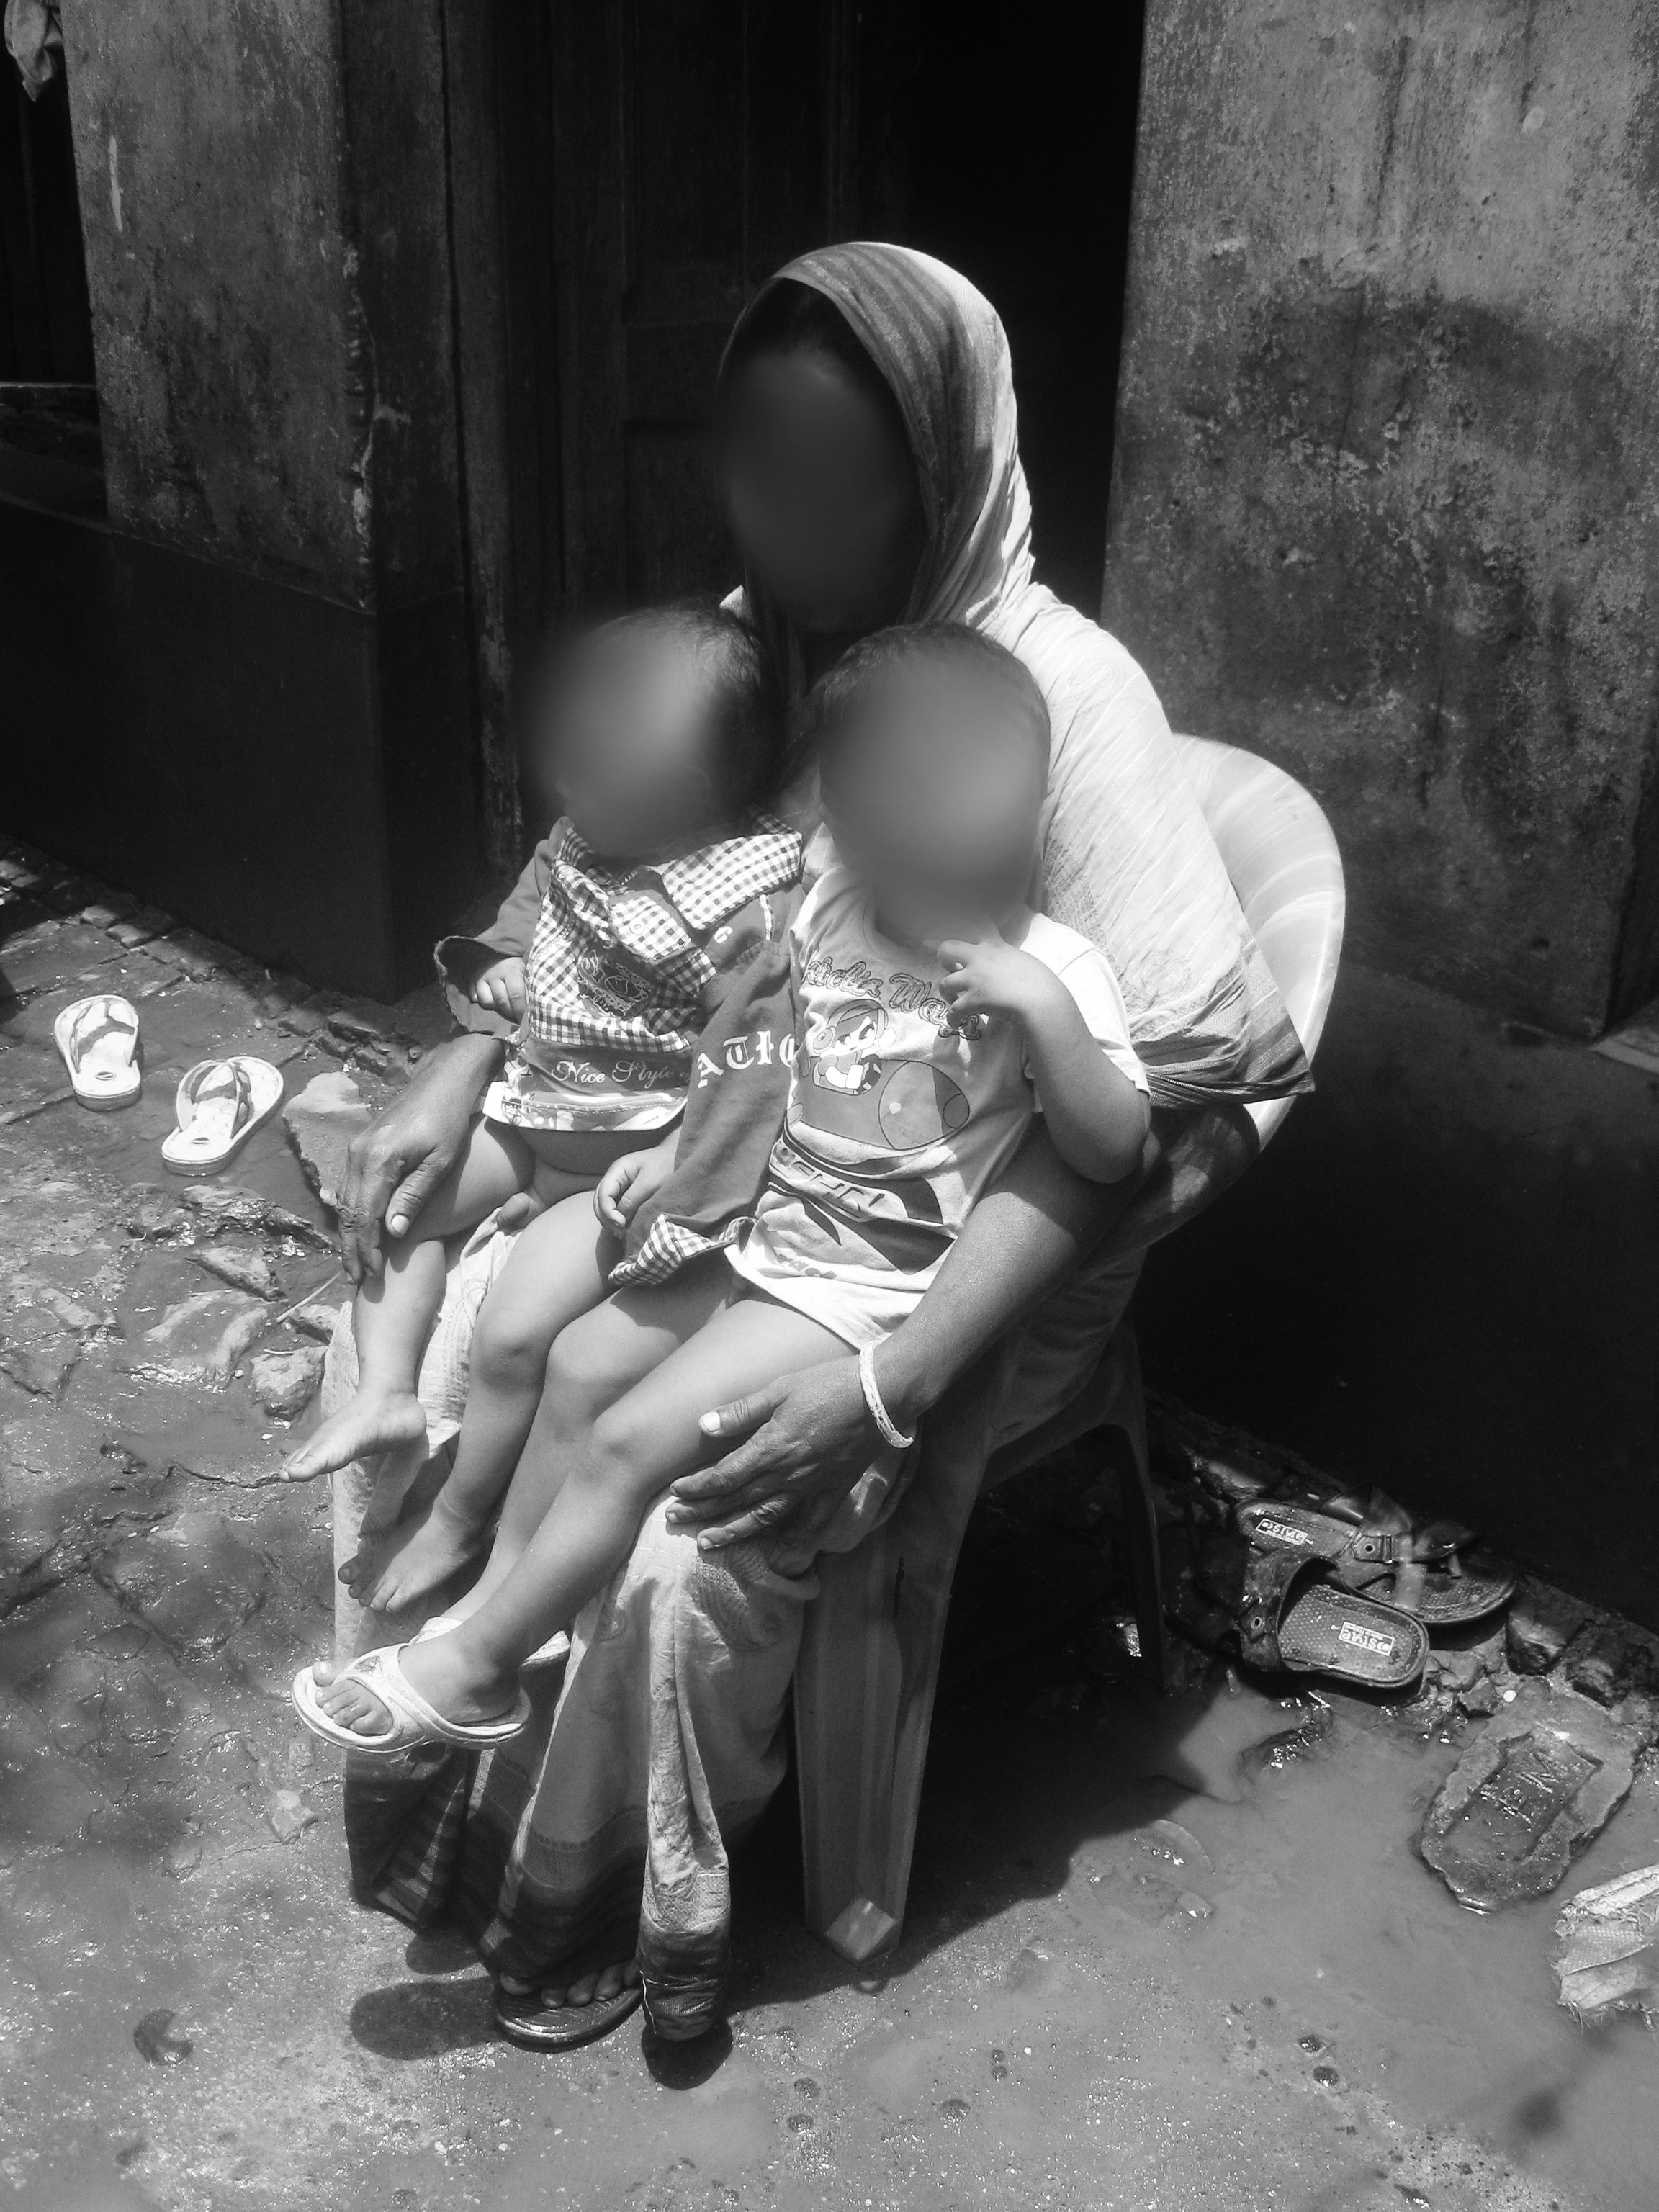
\includegraphics[width=52mm]{manati.jpg}} % Neck figure 
\\[-4mm]
\parbox[t]{52mm}{\Centering\BBI{11.2545}\hspace{1mm}নিগৃহীতার বাচ্চাদের সাথে নিগৃহীতার মা, ছবি জিতেন নন্দীর তোলা। ৪ আগস্ট\hspace{1mm}} % Neck figure caption
\\[-2mm]
\rule{52mm}{1pt}
\end{wraptable}
%
%
%% Reporter's name, place and date of the report.
\BBI{12.2545}৩১ আগস্ট, মহব্বত হোসেন, আকড়া, মহেশতলা\EN{10}\textbullet\\[0.5mm] 
% Body of the reprot
\BN{12.17}কয়েকদিন ধরে আমি আকড়ার তরুণী নিগ্রহের ঘটনায় যারা জেলে রয়েছে, তাদের পরিবারের লোকেদের সঙ্গে কথা বলছি। যে গাড়িতে সেই তরুণীকে নিয়ে যাওয়া হয়েছিল, তার ড্রাইভার ছোট্টু এবং হেল্পার বিজয় মল্লিকের মা ও মাসির সঙ্গে কথা হয়েছে। ওদের কাছ থেকে ঘটনার একটু অন্যরকম একটা ছবি পাওয়া গেছে। তরুণীকে গাড়িতে করে নিয়ে অনেকটা দূরে গিয়ে শেখ সফি, এই ঘটনায় মূল অভিযুক্ত এবং এখনও পলাতক, সে অন্য চারজনকে গাড়ি থেকে নামিয়ে দেয়। এই চারজন একটা মাঠে গিয়ে মদ খায়। সেইসময় সফি গাড়ির মধ্যে কাণ্ডটা ঘটায়। এরপর বাকি চারজন ফিরে এসে মেয়েটাকে পালিয়ে যেতে বলেছিল। কিন্তু সে বলে, চ্ছ্রওকে নিয়ে পালাব'। 

	গাড়ির হেল্পার বিজয় মল্লিকের বাবা অশোক \begin{wraptable}[21]{l}{24mm}
\hfill % For making a blank space at first line of the right column, position of wrap environment is to be selected after initial run. 
\end{wraptable}মল্লিক, মা গীতা মল্লিক, মাসি সীতা মল্লিক। এঁরা সবাই আকড়া স্টেশন চত্বরে মেথরের কাজ করেন। স্টেশনের ২নং প্ল্যাটফর্মেই এঁদের দেখা যায়। স্থায়ী বাসস্থান সেরকম কিছু নেই। মাসি সীতা মল্লিক বলেন, চ্ছ্রআমাদের রেশন কার্ড, প্যান কার্ড, ভোটার কার্ড কিচ্ছু নেই। আমরা এই নোংরা ঘাঁটাঘাঁটি করি। ঘটনার দিন ছোট্টু এসে বিজয়কে বলল, চ্ছ্রচল, একটা ভাড়া আছে, তিনশোটা টাকা পাব। তোকে দেড়শো টাকা দেব।' সেই টাকার লোভে ছেলেটা গাড়িতে গেল হেল্পারি করতে আর ফেঁসে গেল।' 

	১১ আগস্ট সোমবার আলিপুরে মেয়েটাকে নিয়ে গিয়ে ওর গোপন জবানবন্দি নিয়েছেন ম্যাজিস্ট্রেট। তার কয়েকদিন পর টি আই প্যারেডে হাজির করা হয়েছিল আটক চারজনকে। শোনা যাচ্ছে, মেয়েটা সেখানে বলেছে, আসল দোষী এদের মধ্যে নেই।
\end{multicols}
%
\end{minipage}
%
\end{document}
